[101 r\textsuperscript{o}]
\edtext{}{\lemma{permittitur.}\xxref{permi100v}{permi101r}\Afootnote{ \textit{ (1) }\ Hujus rei experimentum capi poterit hoc modo: \textit{(a)}\ Sumatur \textit{(aa)}\ Mercurius\protect\index{Sachverzeichnis}{mercurius|textit} \textit{(bb)}\ liquor aere purgatus, \textit{(aaa)}\ introducatur \textit{(bbb)}\ immittatur ei exigua aeris bullula, sit tubi altitudo quanta maxima commode haberi potest  \textbar\ quam tamen tanto minorem esse sufficit, quanto liquor est gravior, et minimam pro Mercurio\protect\index{Sachverzeichnis}{mercurius|textit} \textit{ erg.}\ \textbar\ ; bulla introducta a liquore expressa liquoris descendere nitentis gravitate\protect\index{Sachverzeichnis}{gravitas|textit} velut elisa locum a liquore replendum implere tentabit \textit{(b)}\ Sumatur Tubus quam longissimus (etsi pro Mercurio\protect\index{Sachverzeichnis}{mercurius|textit} sufficiat minor quam pro aqua) \textit{AB} \textit{(aa)}\ plenus liquo \textit{(bb)}\ clausus in \textit{A} in quem liquor (ut Mercurius\protect\index{Sachverzeichnis}{mercurius|textit}) immittatur per \textit{(aaa)}\ vas apertum \textit{(bbb)}\ orificium apertum sursum conversum \textit{B} ita tamen ut tubus multum absit a pleno si invertatur Tubus ita ut orificium  \textbar\ \textit{B} \textit{ erg.}\ \textbar\ intret in vas eodem liquore stagnans \textit{C}. 
Si Mercurius\protect\index{Sachverzeichnis}{mercurius|textit} \textit{(aaaa)}\ fuit aqua purgatus \textit{(bbbb)}\ aere purgatus non est, delabetur in vas \textit{C} nec nisi 27 circiter pollicibus  \textbar\ qui repraesententur altitudine \textit{BD} \textit{ erg.}\ \textbar\ ultra ejus superficiem eminebit, \textit{(aaaaa)}\ sin aere purgatus sit totus suspensus manebit, nisi forte Tubi \textit{(bbbbb)}\ locus autem in Tubo \textit{AD} ad sensum vacuus, reapse aere ex corpore Mercurii\protect\index{Sachverzeichnis}{mercurius|textit} (ere non purgati) expresso impletus erit, sed eo dilatato seu rarefacto, quod ex eo colligi potest quia aer externus \textbar\ mox \textit{ gestr.}\ \textbar\ foramine in \textit{A} aperto, (ut si vesica obligatam sit, quae acicula perforetur) irrumpit; tum quia aeris externi pressio\protect\index{Sachverzeichnis}{pressio!aeris|textit} Mercurium\protect\index{Sachverzeichnis}{mercurius|textit} ad locum replendum sursum repellere conatur, quod non faceret si is a tergo aeque seu in Tubo ac ante se seu extra tubum aerem aequalis pressionis seu Elaterii\protect\index{Sachverzeichnis}{elaterium|textit} haberet. Hinc sequitur etiam non posse Mercurium\protect\index{Sachverzeichnis}{mercurius|textit} suspensum praecise aequiponderare massae\protect\index{Sachverzeichnis}{massa|textit} aereae in aere libero, aut Elaterio\protect\index{Sachverzeichnis}{elaterium|textit} seu pressioni aeris\protect\index{Sachverzeichnis}{pressio!aeris|textit} clausi, \textit{(aaaaa-a)}\ nisi ei adjiciatur \textit{(bbbbb-b)}\ sed detrahendam esse ab ejus pondere vim funiculi\protect\index{Sachverzeichnis}{funiculus|textit} seu \textit{(aaaaa-aa)}\ vim qua aer \textit{(bbbbb-bb)}\ Elaterium\protect\index{Sachverzeichnis}{elaterium|textit} quo \textbar\ aeris \textit{ gestr.}\ \textbar\  in \textit{(aaaaa-aaa)}\ Tubo \textit{(bbbbb-bbb)}\ loco per descensum vacuato nimis dilatatus se contrahere nititur, \textit{(ccccc)}\ nisi ei addatur pondus aeris\protect\index{Sachverzeichnis}{pondus!aeris|textit} in Tubo post tergum relicti \textit{DA}. Quod si jam aer Elaterio\protect\index{Sachverzeichnis}{elaterium|textit} proprio se expandere potest in infinitum, (modo scilicet nihil sit quod eum comprimat,) ita ut \textit{(aaaaa-a)}\ gutta \textit{(bbbbb-b)}\ bulla exigua aeris implere seu  \textbar\ (in Recipiente exhausto) \textit{ erg.}\ \textbar\  tendere possit vesicam diametri quantaecunque; eadem evenient, quantacunque sit Tubi altitudo, et quantulacunque bulla aeris in liquore relicta, aut ei immissa sit, sufficiet enim loco in Tubo Vacuo relicto quantocunque implendo et Mercurius\protect\index{Sachverzeichnis}{mercurius|textit} semper descendet ad altitudinem usque consuetam. Quodsi aliquando aer ad terminos pervenit ultra quos expandi non potest  \textbar\ aut non facile potest, id est si aer resistit dilatanti, (quod hactenus deprehendi non potuit) uti resistit comprimenti \textit{ erg.}\ \textbar\ , potest tubus tam longus cogitari (etsi incertum hactenus an et opere obtineri) ut Mercurius\protect\index{Sachverzeichnis}{mercurius|textit} descendere non possit, sed ita suspensus maneat  \textbar\ altius solito \textit{ erg.}\ \textbar\ ,  \textit{(aaaaa-aa)}\ ne aerem ultra debitam dilatet \textit{(bbbbb-bb)}\ ne longius descendendo spatium justo majus \textit{(aaaaa-aaa)}\ a tergo relinquat aeremve \textit{(bbbbb-bbb)}\ in Tubo aeremque qui implere debet nimis dilatet. \textit{ (2) }\  Quod aeri quantulocunque facile est, quia quantulacunque aeris guttula in Vacuo \textit{(a)}\ maximam \textit{(b)}\ satis exhausto quantamcunque vesicam tendere potest. Aer enim resistit quidem comprimenti sed non dilatanti, ac dilatari potest in infinitum  \textbar\ quantum sensu judicari queat \textit{ erg.}\ \textbar\ , Elaterio\protect\index{Sachverzeichnis}{elaterium|textit} proprio, id est circulationis generalis omnia in summam subtilitatem  \textbar\ qualis aetheris\protect\index{Sachverzeichnis}{aether|textit} circulantis est \textit{ erg.}\ \textbar\ si possit disjicere conantis, vi, modo scilicet non tantundem alibi comprimatur, nihil enim sine compensatione fieri potest. \textit{ (3) }\ At [...] possit, \textit{(a)}\ supposito quod liquor ipse nihil aliud Elasticum nobis compertum contineat, \textit{(b)}\ nisi [...] liquoris \textbar\ maxima vi \textit{ gestr.}\ \textbar\ eliciatur, [...] intret. \textit{(aa)}\ Sed cur \textit{(bb)}\ Ergo [...] corporis \textbar\ interni \textit{ erg.}\ \textbar\ expressionem [...] est \textit{(aaa)}\ aeris aequipondio in aere \textit{(bbb)}\ ejus [...] insuetae, \textit{(aaaa)}\ aetheris\protect\index{Sachverzeichnis}{aether|textit} circulatio unif \textit{(bbbb)}\ circulatio [...] resistit. \textit{ L}}}
\pagebreak
 \edtext{}{\lemma{}\linenum{|2|||2|}\Afootnote{ad [...] altitudinem \textit{erg. L}}}
                        \edtext{}{\lemma{modo}\linenum{|3|||3|}\Afootnote{\textbar~exigua \textit{gestr.}~\textbar\ ei \textit{L}}}
                        \edtext{}{\lemma{ab}\linenum{|4|||9|}\Afootnote{\textit{ (1) } ipso liquoris lapsu \textit{ (2) } ipsa liquoris gravitate [...] tubi \textbar~et paucitatem aeris intus relicti \textit{erg.} ~\textbar\  pondus [...] tubum \textbar~descensui necessariam \textit{erg.}~\textbar\  non [...] aut \textit{ (a) }  intra \textit{ (b) } ultra [...] rei \textit{ (aa) } rationem \textit{ (bb) } tam elegantis modum, 
                         \textit{L}}}
%Zeitz auskommentiert% \begin{wrapfigure}{l}{0.4\textwidth}        
%\begin{center}            
%               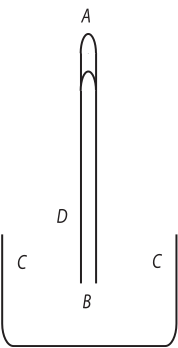
\includegraphics[width=0.18\textwidth]{images/37_3_101r}\\\textit{[Fig. 1, ungestrichen]}
%    \footnote{\textit{Gestrichene Marginalie:} Quare in Vacuo sufficienter exhausto liquor semper descendet ad debitam usque 27 circiter pollicum altitudinem quantulacunque sit tubi longitudo, modo ei aeris bullula suppetat quantulacunque. At in aere ordinario, ubi tantum necesse est ab ipsa liquoris gravitate comprimi aerem extra tubum, quantum relinquendus intra tubum rarefit, fieri potest, ut ob longitudinem tubi et paucitatem aeris intus relicti pondus liquoris ad compressionem aeris extra tubum descensui necessariam non sufficiat, ac proinde aut ultra altitudinem debitam extra liquorem in vase subjecto stagnantem emineat aut etiam quod est mirabilius intra duos aeres suspensum maneat. Cujus rei tam elegantis modum, quia his diebus dum hoc argumentum expendi inveni, nec hactenus extare memini hoc loco proponere decrevi.}
%                %\caption{Bildbeschreibung}
%                        %\end{wrapfigure}      
%                                                     \end{center}  
                       
                       
                       % \edtext{}{\lemma{}\Afootnote{et paucitatem aeris intus relicti \textit{erg. L}}}  
                  %      \edtext{}{\lemma{}\Afootnote{descensui necessariam \textit{erg. L}}}       
                      %  \edtext{}{\lemma{}\Afootnote{\textit{ (a) }  intra \textit{ (b) } ultra \textit{L}}}           
                        %@ @ @ Dies ist eine Abstandszeile - fuer den Fall, dass mehrere figures hintereinander kommen, ohne dass dazwischen laengerer Text steht. Dies kann zu einer Fahlermeldung fuehren. @ @ @ \\
                      %      \edtext{}{\lemma{permittitur.}\xxref{permi100v}{permi101r}\Afootnote{ \textit{ (1) }\ Hujus rei experimentum capi poterit hoc modo:  \textit{(a)}\ Sumatur  \textit{(aa)}\ Mercurius\protect\index{Sachverzeichnis}{mercurius|textit} \textit{(bb)}\ liquor aere purgatus,  \textit{(aaa)}\ introducatur \textit{(bbb)}\ immittatur ei exigua aeris bullula,  sit tubi altitudo quanta maxima commode  haberi potest   \textbar\ quam tamen tanto minorem esse sufficit, quanto liquor est gravior, et minimam pro Mercurio\protect\index{Sachverzeichnis}{mercurius|textit} \textit{ erg.}\ \textbar\ ; bulla introducta a liquore expressa  liquoris descendere nitentis gravitate\protect\index{Sachverzeichnis}{gravitas|textit} velut elisa locum  a liquore replendum implere tentabit \textit{(b)}\ Sumatur Tubus  quam longissimus (etsi pro Mercurio\protect\index{Sachverzeichnis}{mercurius|textit} sufficiat minor quam  pro aqua) \textit{AB}  \textit{(aa)}\ plenus liquo \textit{(bb)}\ clausus in \textit{A}  in quem liquor (ut Mercurius\protect\index{Sachverzeichnis}{mercurius|textit}) immittatur per  \textit{(aaa)}\ vas apertum \textit{(bbb)}\ orificium apertum sursum conversum \textit{B} ita tamen ut tubus multum absit a pleno  si invertatur Tubus ita ut orificium   \textbar\ \textit{B} \textit{ erg.}\ \textbar\  intret in vas eodem  liquore stagnans \textit{C}. Si Mercurius\protect\index{Sachverzeichnis}{mercurius|textit}  \textit{(aaaa)}\ fuit aqua purgatus \textit{(bbbb)}\  aere purgatus non est, delabetur in vas \textit{C} nec  nisi 27 circiter pollicibus   \textbar\ qui repraesententur altitudine \textit{BD} \textit{ erg.}\ \textbar\  ultra ejus superficiem  eminebit,  \textit{(aaaaa)}\ sin aere purgatus sit totus suspensus  manebit, nisi forte Tubi \textit{(bbbbb)}\ locus autem in  Tubo \textit{AD} ad sensum vacuus, reapse aere ex corpore Mercurii\protect\index{Sachverzeichnis}{mercurius|textit} (ere non purgati) expresso impletus erit,  sed eo dilatato seu rarefacto, quod ex eo colligi  potest quia aer externus  \textbar\ mox \textit{ gestr.}\ \textbar\  foramine in \textit{A} aperto, (ut  si vesica obligatam sit, quae acicula perforetur)  irrumpit; tum quia aeris externi pressio\protect\index{Sachverzeichnis}{pressio!aeris|textit} Mercurium\protect\index{Sachverzeichnis}{mercurius|textit}  ad locum replendum sursum repellere conatur, quod  non faceret si is a tergo aeque seu in Tubo ac ante se seu extra tubum aerem aequalis pressionis  seu Elaterii\protect\index{Sachverzeichnis}{elaterium|textit} haberet. Hinc sequitur etiam non posse Mercurium\protect\index{Sachverzeichnis}{mercurius|textit} suspensum praecise aequiponderare massae\protect\index{Sachverzeichnis}{massa|textit}  aereae in aere libero, aut Elaterio\protect\index{Sachverzeichnis}{elaterium|textit} seu pressioni aeris\protect\index{Sachverzeichnis}{pressio!aeris|textit}  clausi,  \textit{(aaaaa-a)}\ nisi ei adjiciatur \textit{(bbbbb-b)}\ sed detrahendam  esse ab ejus pondere vim funiculi\protect\index{Sachverzeichnis}{funiculus|textit} seu  \textit{(aaaaa-aa)}\ vim qua aer \textit{(bbbbb-bb)}\ Elaterium\protect\index{Sachverzeichnis}{elaterium|textit} quo  \textbar\ aeris \textit{ gestr.}\ \textbar\   in  \textit{(aaaaa-aaa)}\ Tubo \textit{(bbbbb-bbb)}\ loco per descensum vacuato nimis dilatatus se  contrahere nititur, \textit{(ccccc)}\ nisi ei addatur pondus aeris\protect\index{Sachverzeichnis}{pondus!aeris|textit} in Tubo  post tergum relicti \textit{DA}. Quod si jam aer Elaterio\protect\index{Sachverzeichnis}{elaterium|textit} proprio se expandere potest in infinitum, (modo scilicet nihil sit quod eum comprimat,)  ita ut  \textit{(aaaaa-a)}\ gutta \textit{(bbbbb-b)}\ bulla exigua aeris implere seu   \textbar\ (in Recipiente exhausto) \textit{ erg.}\ \textbar\   tendere possit vesicam diametri quantaecunque; eadem  evenient, quantacunque sit Tubi altitudo, et quantulacunque  bulla aeris in liquore relicta, aut ei  immissa sit, sufficiet enim loco in Tubo Vacuo  relicto quantocunque implendo et Mercurius\protect\index{Sachverzeichnis}{mercurius|textit} semper descendet  ad altitudinem usque consuetam. Quodsi aliquando aer ad terminos  pervenit ultra quos expandi non potest   \textbar\ aut non facile potest, id est si aer resistit dilatanti, (quod hactenus deprehendi non potuit) uti resistit comprimenti \textit{ erg.}\ \textbar\ , potest tubus tam  longus cogitari (etsi incertum hactenus an et opere obtineri)  ut Mercurius\protect\index{Sachverzeichnis}{mercurius|textit} descendere non possit,  sed ita suspensus  maneat   \textbar\ altius solito \textit{ erg.}\ \textbar\ ,   \textit{(aaaaa-aa)}\ ne aerem ultra debitam dilatet \textit{(bbbbb-bb)}\  ne longius descendendo spatium justo majus  \textit{(aaaaa-aaa)}\ a tergo relinquat  aeremve \textit{(bbbbb-bbb)}\ in Tubo aeremque qui implere debet nimis dilatet. \textit{ (2) }\   Quod aeri quantulocunque facile est, quia quantulacunque  aeris guttula in Vacuo  \textit{(a)}\ maximam \textit{(b)}\ satis exhausto quantamcunque  vesicam tendere potest. Aer enim resistit quidem comprimenti  sed non dilatanti, ac dilatari potest in infinitum   \textbar\ quantum sensu judicari queat \textit{ erg.}\ \textbar\ , Elaterio\protect\index{Sachverzeichnis}{elaterium|textit}  proprio, id est circulationis generalis omnia in summam  subtilitatem   \textbar\ qualis aetheris\protect\index{Sachverzeichnis}{aether|textit} circulantis est \textit{ erg.}\ \textbar\  si possit disjicere conantis, vi, modo scilicet  non tantundem alibi comprimatur, nihil enim sine compensatione fieri potest. \textit{ (3) }\ At [...] possit, \textit{(a)}\ supposito  quod liquor ipse nihil aliud Elasticum nobis compertum  contineat, \textit{(b)}\ nisi [...] liquoris  \textbar\ maxima vi \textit{ gestr.}\ \textbar\ eliciatur, [...] intret. \textit{(aa)}\ Sed cur \textit{(bb)}\ Ergo [...] corporis  \textbar\ interni \textit{ erg.}\ \textbar\ expressionem [...] est \textit{(aaa)}\ aeris aequipondio in  aere \textit{(bbb)}\ ejus [...] insuetae, \textit{(aaaa)}\ aetheris\protect\index{Sachverzeichnis}{aether|textit} circulatio unif \textit{(bbbb)}\ circulatio [...] resistit. \textit{ L}}}